\documentclass[a4paper,onecolumn]{article}
\usepackage{amsmath, amsthm, graphicx, amssymb, wrapfig, fullpage, subfigure, array}
\usepackage[font=sl, labelfont={sf}, margin=1cm]{caption}
\DeclareMathOperator{\e}{e}
\begin{document}
\setcounter{page}{1}

\section{Example: Oil Reservoir Optimal Control}
\begin{figure}[h]
\begin{center}
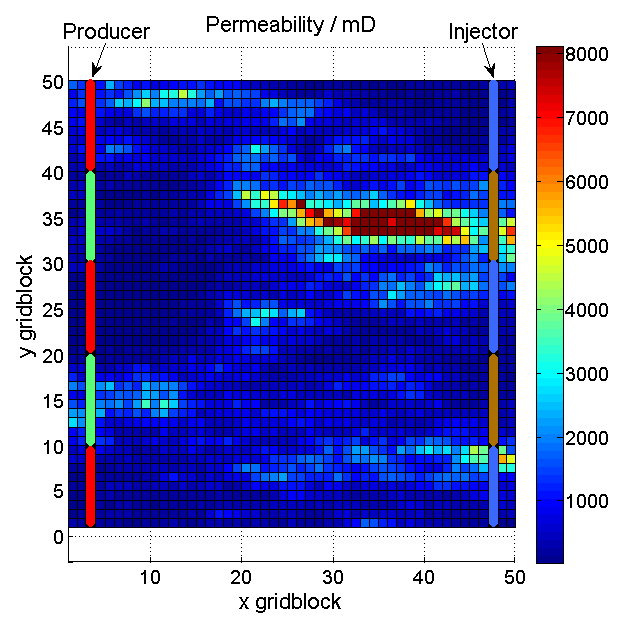
\includegraphics[width=6cm,angle=90]{Permeability.png}
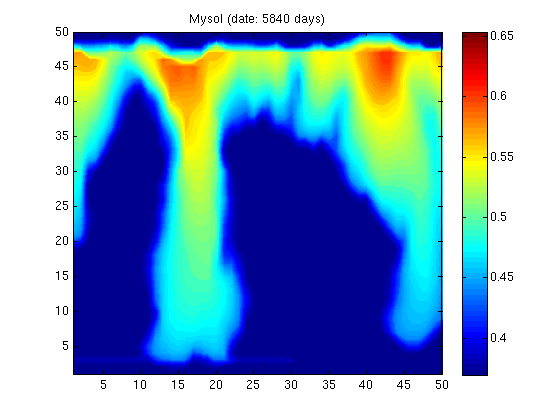
\includegraphics[width=7cm]{mysol_5840.png}
\end{center}
\end{figure}


\section{Problem Setup}
Consider a optimal control problem
\begin{equation}\left\{
\begin{split}
  \dot{x} &= F(x,\xi, u)\\
  y &= g(x) \quad [+\epsilon]
\end{split}
\right.
\end{equation}
with initial condition $x(0) = x_0$. $x\in \mathbb{R}^n$, $y\in
\mathbb{R}^m$, $\xi\in\mathbb{R}^n$, $m<n$. $\xi$ is the fixed but unknown. 
Objective is to maximize
\begin{equation}
    J_T = \int_0^T e^{-t\gamma}\phi(x,u) \textrm{d}t
\end{equation}
At $t=0$, the prior on $\xi$ can be modelled by a set of particles
$\xi_1, \cdots, \xi^N$. 
If a myopic approach is adopted, the optimal control will be
\begin{equation}
    u^* = \arg\min_u \frac{1}{N}\sum_i J_T\left(x(u,\xi^i;x_0), u
	\right)\,,
\end{equation}
which is equivalent to no observation.\\

\noindent The first approach we thought of is poMDP. We assume $T=
\infty$.
We discretize time into $t_0=0, t_1, \cdots $.
If we accounts for the effect of future observations, we use Bellman's
equation\footnote{Warren B. Powell, Approximate Dynamics Programming:
Solving the Curses of Dimensionality}
\begin{equation}\begin{split}
  u_t^*(S_t) &= \arg\max_{u_t} \mathbb{E}\left[\left(\phi(x, u_t)\Delta
  t+ e^{-\Delta t \gamma}
  V(S_{t+1})\right)\right]\\
  V(S_t) &= \mathbb{E}\left[\left(\phi(x, u^*_t)\Delta
    t+ e^{-\Delta t \gamma}
	  V(S_{t+1})\right)\right]\\
  S_{t+1} &= S_{t+1}(S_t, u_t)
\end{split}\end{equation}
$S_t$ is the belief state, i.e. the probability measure of $(\xi,x)$, at $t$.
Notice: not like poMDP, the transition from $S_t$ to $S_{t+1}$ is
deterministic for a fixed $u_t$.\\

\section{A Tentative Alternative Approach?}


\end{document}








